%\appendix
%\appendixpage

\section*{Appendix}
%\label{sec:ap}

To illustrate the inner workings of the proposed algorithm on a variety of problems, for a single replication of each of the four data sets in Section~\ref{sec:real-data} we recorded the number of features discarded by each screening method at each $\lambda$ value along the path of $L=100$ values. Features discarded by SEDPP are safely discarded, while features discarded by SSR are not necessarily safe and require additional checks. For the adaptive hybrid rule, we use AHR\_Safe to denote the features that are safely discarded first by adaptive EDPP and AHR\_Strong to denote features that discarded afterward by adaptive SSR and require additional checks. The results are summarized in Figure \ref{fig:ap1}.

\begin{figure}[H]
    \centering
    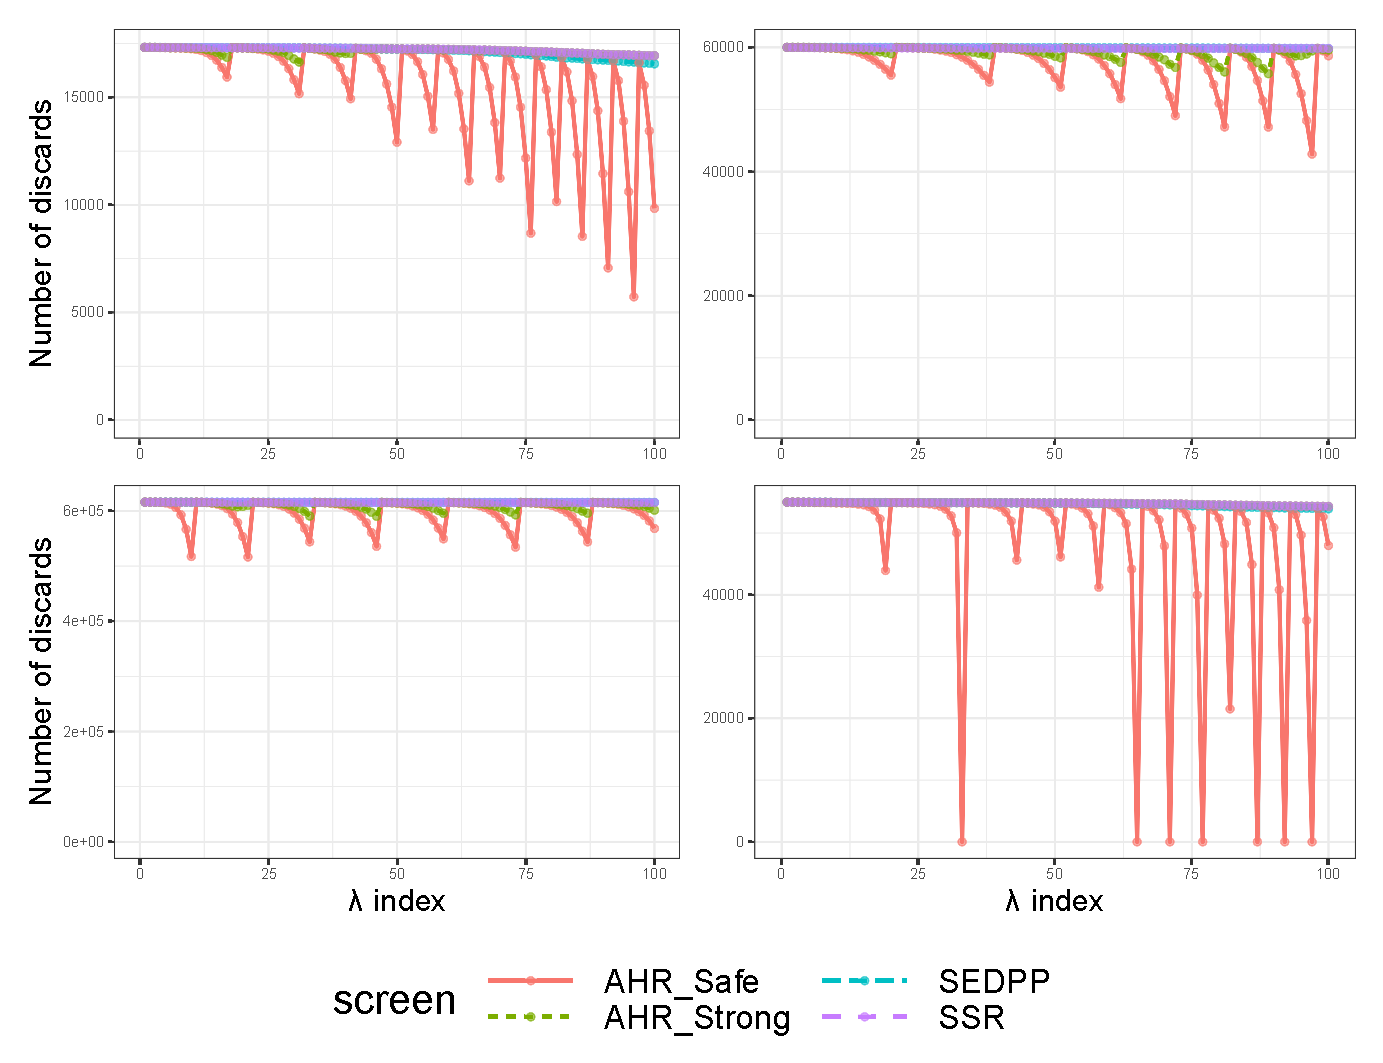
\includegraphics[width=0.82\textwidth]{app1.eps}    \caption{Comparing number of discards by screening methods for lasso model along $\lambda$ values.}
    \label{fig:ap1}
\end{figure}

Note that the AHR method is rather ``jumpy''; this is by design, and these spikes represent moments along the path that triggered an update of the reference solution to gain more screening power. Our adaptive updating algorithm determines the timing of update dynamically depending on the screening performance. For all four data sets, with about only 10 updates, the adaptive hybrid screening can safely discard a great number of features at most $\lambda$ values.

Next we compare the number of rounds of KKT condition checks and the number of KKT condition checks on individual features needed for AHR and SSR respectively, as shown in Table \ref{Tab:kkt1} and Table \ref{Tab:kkt2}. In a round of KKT condition checking, all features that are not discarded by the safe rule are checked, which potentially includes a large number of individual feature checks.

\begin{table}[H]
\centering
\begin{tabular}{lllll}
\toprule
Screening method & GENE & MNIST & GWAS & NYT \\
\midrule
SSR & 99 & 99 & 99 & 99 \\
AHR & 99 & 99 & 99 & 99 \\
\bottomrule
\end{tabular}
\caption{Number of rounds of KKT conditions checks required for the whole path}
\label{Tab:kkt1}
\end{table}

\begin{table}[H]
\centering
\begin{tabular}{lllll}
\toprule
Screening method & GENE & MNIST & GWAS & NYT \\
\midrule
SSR & 1,712 & 5,943 & 60,986 & 5,429 \\
AHR & 172 & 286 & 2,353 & 622 \\
\bottomrule
\end{tabular}
\caption{Number of KKT conditions checks on individual features ($\times10^3$) required for the whole path}
\label{Tab:kkt2}
\end{table}

Although all paths includes $L=100$ $\lambda$ values, the solution at the first value is exactly $\hat{\beta}(\lambda_0)=0$ and does not require any checking. Thus, if no violations occur in the application of the strong rule, the number of rounds of KKT condition checking required will attain its minimum value of $99$. In all four data sets, neither SSR nor the adaptive SSR in AHR is ever violated (as other authors have discussed, violations are rare but possible). However, the two methods are very different in terms of the number of individual features involved in these condition checks. AHR requires far fewer checks on individual features because the adaptive EDPP narrows down the set of features that need to be checked by an order of magnitude, which is how it achieves greater computational efficiency.
